% Response diagram for examiner Q1
\documentclass[tikz,border=12pt]{standalone}
\usepackage[T1]{fontenc}
\usepackage{lmodern}
\usepackage{tikz}
\usetikzlibrary{positioning,fit,arrows.meta,calc}

\tikzset{
  every node/.style={font=\sffamily},
  blk/.style={
    draw=black!70, rounded corners=4pt, line width=0.8pt,
    fill=white, align=center, inner sep=8pt,
    text width=10.5cm, font=\normalsize
  },
  zone/.style={
    draw=black!55, rounded corners=6pt, line width=0.9pt,
    inner sep=12pt, fill=#1
  },
  role/.style={
    draw=black!55, line width=1pt, rounded corners=4pt,
    fill=#1, align=left, inner sep=7pt,
    text width=5.0cm, font=\small
  },
  arr/.style={->, >=Latex, line width=1pt, draw=black!70},
  trust/.style={->, >=Latex, line width=1pt, draw=blue!60!black},
  dep/.style={->, >=Latex, line width=1pt, draw=orange!70!black, dashed}
}

\begin{document}
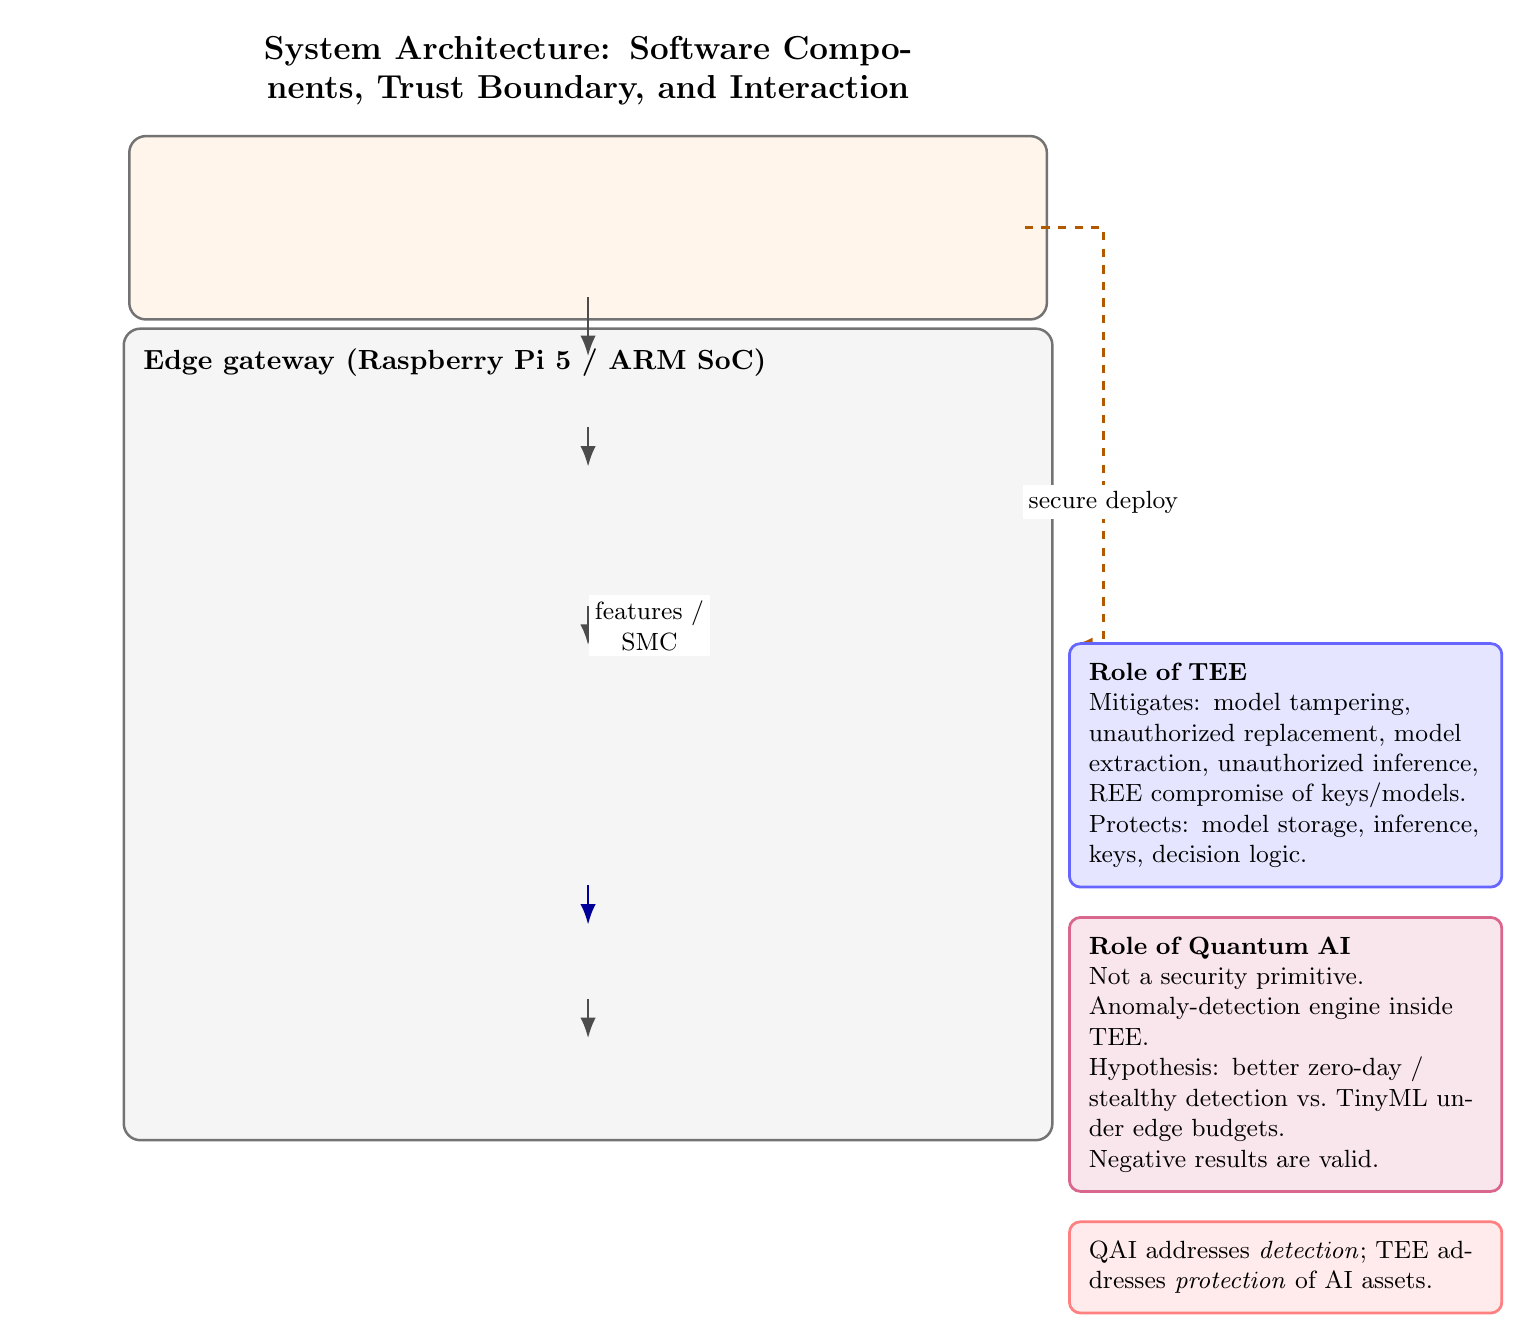
\begin{tikzpicture}[node distance=0.5cm]

\node[font=\bfseries\large, align=center, text width=14cm] (title) at (0,0)
  {System Architecture: Software Components, Trust Boundary, and Interaction};

\node[blk, fill=orange!10, below=0.55cm of title] (train) {%
  \textbf{Development host / cloud (offline)}\\
  Datasets $\rightarrow$ PyTorch (TinyML baseline) $\rightarrow$ Qiskit + PennyLane\\
  $\rightarrow$ compression \& export $\rightarrow$ signed encrypted model bundle};

\node[zone=orange!8, fit=(train), inner sep=8pt] {};

\node[blk, fill=green!8, below=0.75cm of train] (iot)
  {IoT devices $\rightarrow$ Data collection layer};

\node[blk, fill=red!8, below=of iot] (ree) {%
  \textbf{Linux OS — REE (attack surface)}\\
  Network stack, management agent, feature extraction, TEE Client API};

\node[blk, fill=blue!8, below=of ree, minimum height=2.8cm] (tee) {%
  \textbf{TEE — OP-TEE / ARM TrustZone (protected)}\\
  Secure Key Storage \textbar\ Trusted AI Model Storage \textbar\ Trusted Inference TA\\
  Remote Attestation Service\\
  \rule{9.5cm}{0.4pt}\\
  Hybrid Quantum--Classical Detection Engine (compressed runtime)};

\node[blk, fill=blue!8, below=of tee] (dec)
  {Security decision logic $\rightarrow$ alerts / policy actions};

\node[blk, fill=cyan!8, below=of dec] (cloud)
  {Cloud management / monitoring, attestation verifier};

\node[zone=gray!8, fit=(iot)(cloud), inner sep=10pt] (edge) {};
\node[font=\bfseries, anchor=north west] at ([xshift=4pt,yshift=-4pt]edge.north west)
  {Edge gateway (Raspberry Pi 5 / ARM SoC)};

\draw[arr] (train.south) -- (iot.north);
\draw[arr] (iot) -- (ree);
\draw[arr] (ree) -- node[font=\small, fill=white, inner sep=2pt, right, align=center]
  {features /\\SMC} (tee);
\draw[trust] (tee) -- (dec);
\draw[arr] (dec) -- (cloud);
\draw[dep] (train.east) -- ++(1.0,0) |- node[font=\small, fill=white, inner sep=2pt, pos=0.35, above]
  {secure deploy} ([xshift=0.6cm]tee.east |- tee.north);

\node[role=blue!10, draw=blue!60, right=0.55cm of tee] (teerole) {%
  \textbf{Role of TEE}\\
  Mitigates: model tampering, unauthorized replacement, model extraction, unauthorized inference, REE compromise of keys/models.\\
  Protects: model storage, inference, keys, decision logic.};

\node[role=purple!10, draw=purple!60, below=0.35cm of teerole] (qairole) {%
  \textbf{Role of Quantum AI}\\
  Not a security primitive. Anomaly-detection engine inside TEE.\\
  Hypothesis: better zero-day / stealthy detection vs.\ TinyML under edge budgets.\\
  Negative results are valid.};

\node[role=red!8, draw=red!50, below=0.35cm of qairole] (note) {%
  QAI addresses \emph{detection}; TEE addresses \emph{protection} of AI assets.};

\end{tikzpicture}
\end{document}
